\documentclass[12pt]{article}

\usepackage{sbc-template}
\usepackage{graphicx,url}
\usepackage{float}
\usepackage[utf8]{inputenc}
\usepackage[brazil]{babel}
\usepackage[latin1]{inputenc}  

     
\sloppy

\title{Simulated Annealing\\ Uma resolução para SAT-3}

\author{César Eduardo de Souza\inst{1},\\ Guilherme Diel\inst{1}}


  \address{Departamento de Ciência da Computação \\ Universidade do Estado de Santa Catarina
  (UDESC) -- Joinville, SC -- Brazil
  \email{\{cesar.souza, guilherme.diel\}@edu.udesc.br}
}

\begin{document} 

\maketitle

     
\begin{resumo} 
  Resumo
\end{resumo}


\section{Introdução}
\label{sec:introducao}
% Contextualização do problema/tarefa e revisão da literatura.

Foi no século XX que se iniciou a busca pela resolução de problemas NP, NP-Hard e NP-Completo usando ferramentas computacionais. 
%
Estas portanto, foram, em sua maioria, desenvolvidos com base em algoritmos heurísticos – alicerçados em técnicas de busca de solução não necessariamente ótima, mas sim satisfatória –. 
%
Sendo assim, alguns destes tornaram-se mais disseminados na literatura científica, como a \textbf{Busca Gulosa}, \textbf{Algoritmo A*}, \textbf{Subida de Encosta} e \textbf{Simulated Annealing}. 

O método de \textbf{Simulated Annealing} teve sua lógica concebida a partir do método de anelização de materiais, Metropolis, desenvolvido por Gibbs em 1953 \cite{metropolis1953equation}.
%
Basado na fabricação de aneis, este método usa como base o fato de que, quanto mais quente está o material, maior se torna a facilidade de modelá-lo.
%
Sob o mesmo ponto de vista, este método consiste em uma sequencia de temperaturas decrescentes em que, quanto maior a temperatura atual, mais aleatorizada são as otimizações geradas pelo algoritmo, sendo que, quando a temperatura chegar a um certo ponto idealizando a otimização do resultado conforme decresce a temperatura, até que esta se torne mínima.

Um problema muito conhecido e discutido na literatura, que é capaz de ser resolvido por algoritmos heuristicos, é o problema da satisfabilidade (SAT), que consiste em, dado um conjunto de cláusulas disjuntivas na forma normal conjuntiva, determinar se existe uma atribuição de valores lógicos (\textit{verdadeiro} ou \textit{falso}) às variáveis envolvidas que satisfaça toda a expressão.
%
Cada cláusula é composta por uma disjunção (operador lógico $\lor$) de literais (variáveis ou suas negações), e a fórmula booleana global é uma conjunção (operador lógico $\land$) dessas cláusulas. Formalmente:

\begin{equation}
\bigwedge_{i=1}^{m} \left( \bigvee_{j=1}^{k} l_{ij} \right)
\end{equation}

Ao longo deste relatório, será abordado uma proposta de implementação de do \textbf{Simulated Annealing} para resolução de uma variante do SAT, conhecido como SAT-3, que consiste em três variáveis por cláusula no problema SAT.

Este relatório está organizado da seguinte maneira: a seção 2 apresenta estratégias utilizadas, descrições, justificativas de escolhas, fórmulas utilizadas e descrições. Em seguida, na seção 3 são abordadas descrições dos experimentos, configurações utilizadas e descrições dos resultados obtidos. Outrossim, na seção 4 expõem-se considerações sobre os resultados obtidos e análises críticas sobre os mesmos. Por fim, na seção 5 mostra-se considerações sobre o trabalho desenvolvido e identificação de direcionamentos futuros na pesquisa.


% Justificativa e motivação.
% Objetivo.
% Organização do texto.

\section{Metodologia de Desenvolvimento}
\label{sec:metodologia_de_desenvolvimento}

O método de \textbf{Simulated Annealing} consiste em:
\begin{enumerate}
  
  \item Para uma temperatura $T_i$, realizar $N$ vezes: \label{passo:1}
  \begin{itemize}
    \item Realizar uma perturbação aleatória no estado atual $\text{estado}_0$, gerando um novo $\text{estado}_i$
    \item Calcular a variação de energia $\Delta E = E(\text{estado}_i) - E(\text{estado}_0)$
    \item Se $\Delta E < 0$ (melhora na energia), aceitar a transição ($\text{estado}_i \rightarrow \text{estado}_0$)
    \item Caso contrário, aceitar a transição com probabilidade P_{\text{accept}}($T_i$)
  \end{itemize}
  
  \item Critério de parada:
  \begin{itemize}
    \item Se $T_i \leq T_f$ (temperatura final) ou o sistema atingir convergência (e.g., $\Delta E \approx 0$ por $k$ iterações consecutivas)
    \item Retornar o $\text{estado}_0$ como solução
    \item Caso contrário, reduzir a temperatura ($T_i \leftarrow \alpha T_i$, com $0 < \alpha < 1$) e retornar ao Passo~\ref{passo:1}
  \end{itemize}
  \label{pseudocodigo}
  \caption{Passo a passo do método de \textbf{Simulated Annealing}}
\end{enumerate} 

A aplicação do método de \textbf{Simulated Annealing} para a otimização do problema do SAT-3 foi realizada por meio da linguagem de programação \textit{Python}, junto com a biblioteca \textit{Numpy}.
%
A Figura \ref{fig:metodologia} retrata o passo a passo de como foi implementado este algoritmo.
%
O passo 1 (inicialização) consiste em realizar a inicialização do sistema:

\begin{itemize}
  \item Temperatura inicial $T_0$ = 1000
  \item Taxa de resfriamento \alpha = 0.99
  \item Temperatura final $T_f$ = 0.1
  \item Número de iterações por temperatura $N$ = 1000
\end{itemize}

No segundo passo (iteração por temperatura) da Figura \ref{fig:metodologia} a fórmula de probabilidade de aceitação de estados com pior energia que foi adotada, foi:
\begin{equation}
  P_{\text{accept}} = \exp\left(-\frac{\Delta E}{T_i}\right)
\end{equation}

O terceiro passo (resfriamento) corresponde ao passo \ref{passo:1} do codigo de \ref{pseudocodigo}.

\begin{figure}[H]
  \centering
  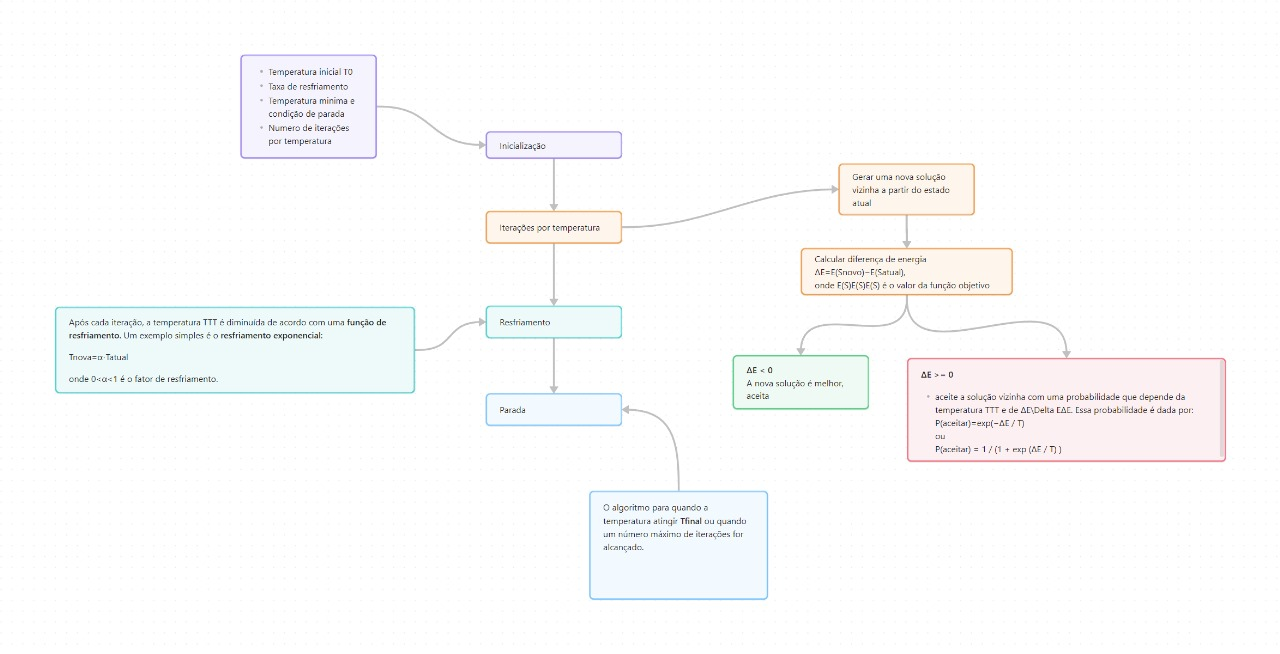
\includegraphics[width=1\textwidth]{pasta_.jpeg}
  \caption{Diagrama do algoritmo de \textbf{Simulated Annealing}}
  \label{fig:metodologia}
  \end{figure}
% descrições e justificativas das escolhas.
% Fórmulas utilizadas, descrições e justificativas.

\section{Descrição de Experimentos/Simulações e Resultados Obtidos}
\label{sec:descicao_de_experimentos_/_simulacoes_e_resultados_obtidos}

% Descrição dos experimentos
% e configurações utilizadas.

Foi com a temperatura inicial = 1000 = iterações por temperatura taa de resfriamento = 0.99 

% Descrição dos resultados obtidos (Figuras, Tabelas, Gráficos).

Nestas configurações foram obtidos resultados para bases de SAT-3 de 20, 100 e 250 entradas como os seguintes gráficos de convergência:% to pensando em fazer o \ref pra cada um mas sla tb

\begin{figure}[H]
  \centering
  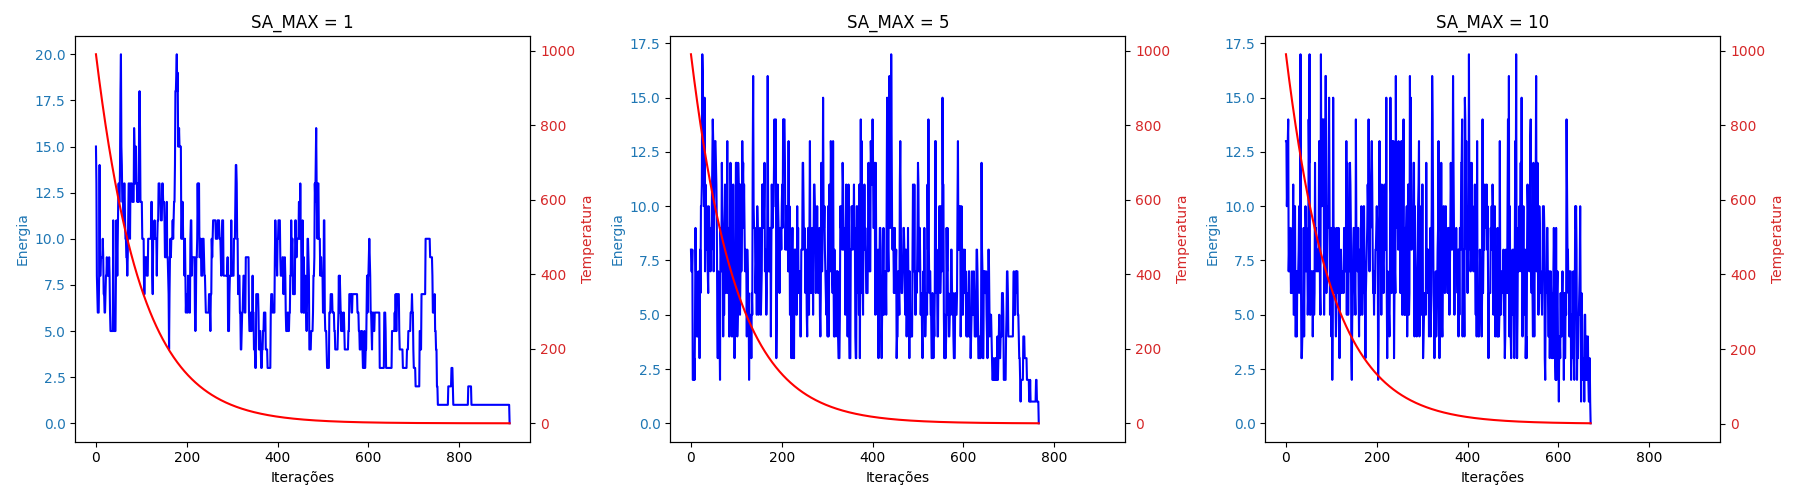
\includegraphics[width=.9\textwidth]{../../melhores_sa_20.png}
  \caption{Convergência para 20 entradas}
  \label{fig:metodologia}
  \end{figure}

\begin{figure}[H]
  \centering
  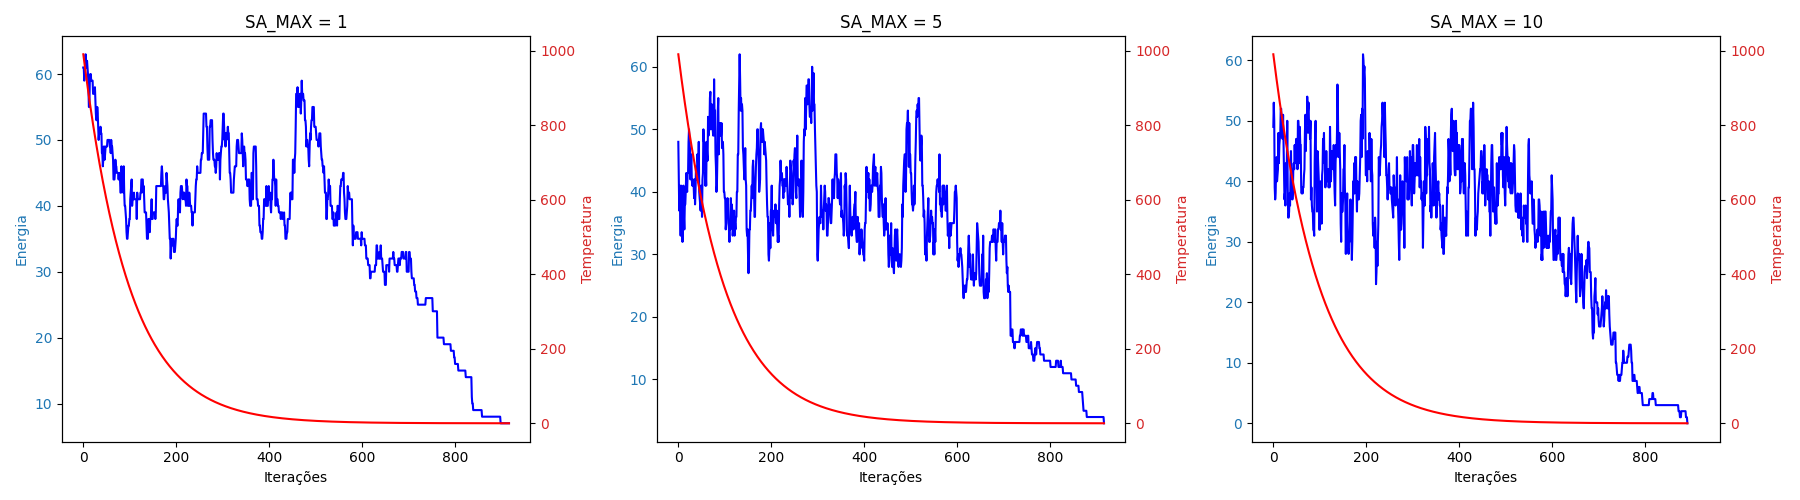
\includegraphics[width=.9\textwidth]{../../melhores_sa_100.png}
  \caption{Convergência para 100 entradas}
  \label{fig:metodologia}
   \end{figure}

\begin{figure}[H]
  \centering
  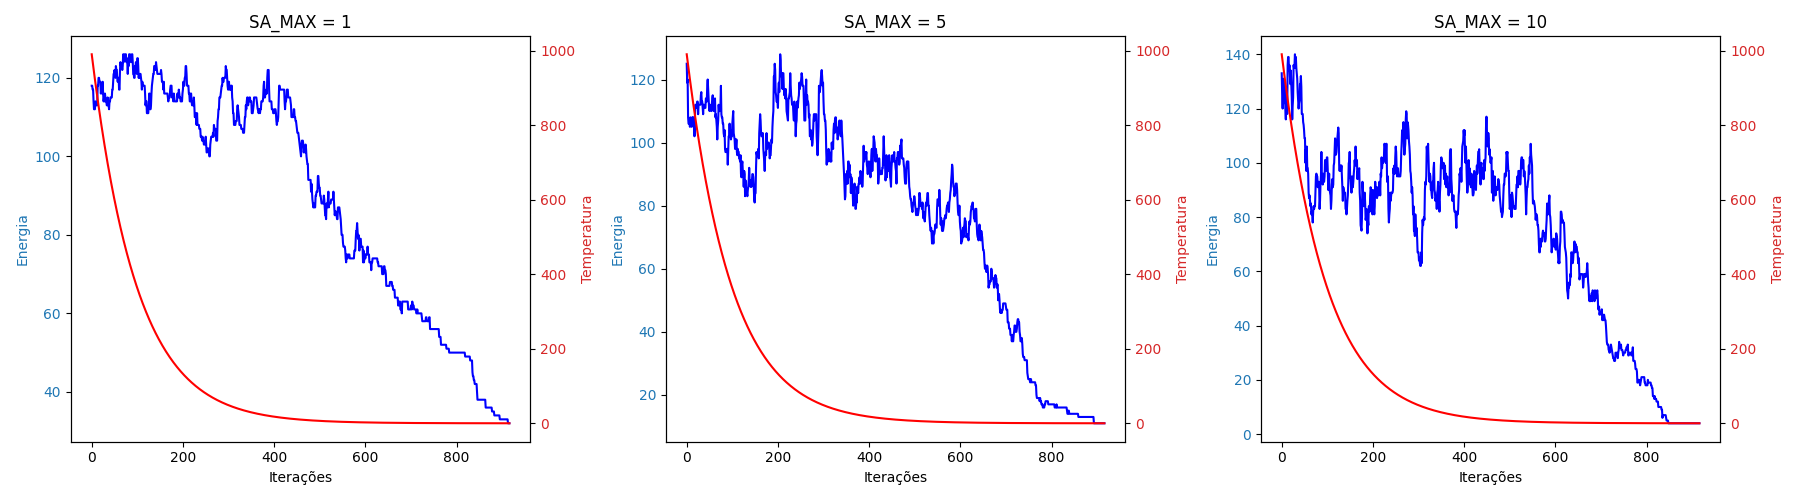
\includegraphics[width=.9\textwidth]{../../melhores_sa_250.png}
  \caption{Convergência para 250 entradas}
  \label{fig:metodologia}
  \end{figure}


Além disso, é possível verificar a seguinte tabela com média e desvio padrão de 30 execuções do experimento, apontados pelos consecutivos boxplots.

\begin{table}[H]
\centering
\caption{Média e Desvio Padrão dos Resultados Obtidos}
\begin{tabular}{|c|c|c|c|}
\hline
\textbf{SAMAX} & \textbf{Número de Entradas} & \textbf{Média} & \textbf{Desvio Padrão} \\ \hline
1   & 20 & 0.80 & 0.85 \\ \hline
5   & 20 & 0.17 & 0.53 \\ \hline
10  & 20 & 0.03 & 0.18 \\ \hline
1   & 100 & 12.43 & 3.09 \\ \hline
5   & 100 & 5.67 & 1.56 \\ \hline
10  & 100 & 3.93 & 1.48 \\ \hline
1   & 250 & 43.53 & 6.25 \\ \hline
5   & 250 & 16.10 & 3.29 \\ \hline
10  & 250 & 9.93 & 2.48 \\ \hline

\end{tabular}
\label{tab:resultados}
\end{table}

\begin{table}[H]
  \centering
  \caption{Média e Desvio Padrão do Histórico dos Resultados Obtidos}
  \begin{tabular}{|c|c|c|c|}
    \hline
    \textbf{SAMAX} & \textbf{Número de Entradas} & \textbf{Média} & \textbf{Desvio Padrão} \\ \hline
    1   & 20 & 6.50 & 3.47 \\ \hline
    5   & 20 & 7.18 & 3.39 \\ \hline
    10  & 20 & 7.34 & 3.22 \\ \hline
    1   & 100 & 35.14 & 11.74 \\ \hline
    5   & 100 & 31.41 & 13.39 \\ \hline
    10  & 100 & 30.70 & 14.16 \\ \hline
    1   & 250 & 90.75 & 23.46 \\ \hline
    5   & 250 & 78.44 & 30.06 \\ \hline
    10  & 250 & 75.82 & 32.76 \\ \hline
  
  \end{tabular}
  \label{tab:resultados}
  \end{table}


\begin{figure}[H]
  \centering
  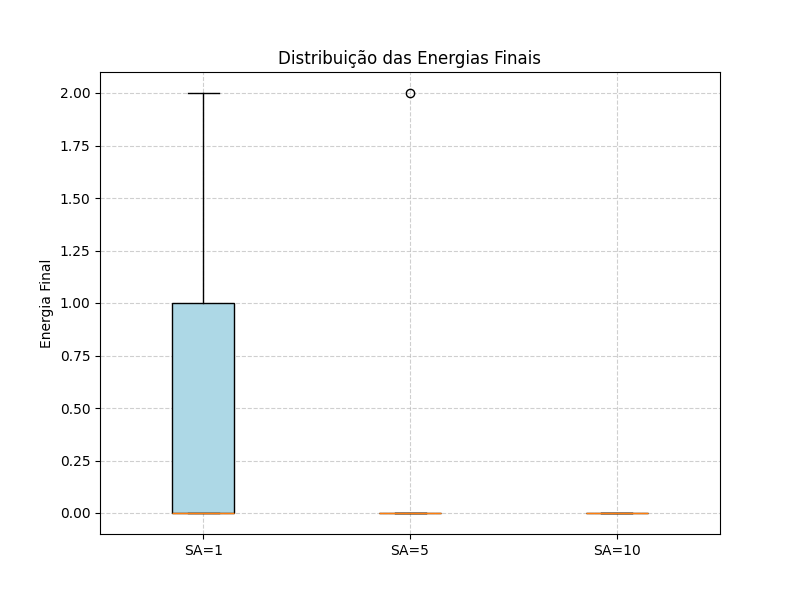
\includegraphics[width=.9\textwidth]{../../boxplot_20.png}
  \caption{Boxplots para 20 entradas}
  \label{fig:metodologia}
  \end{figure}

\begin{figure}[H]
  \centering
  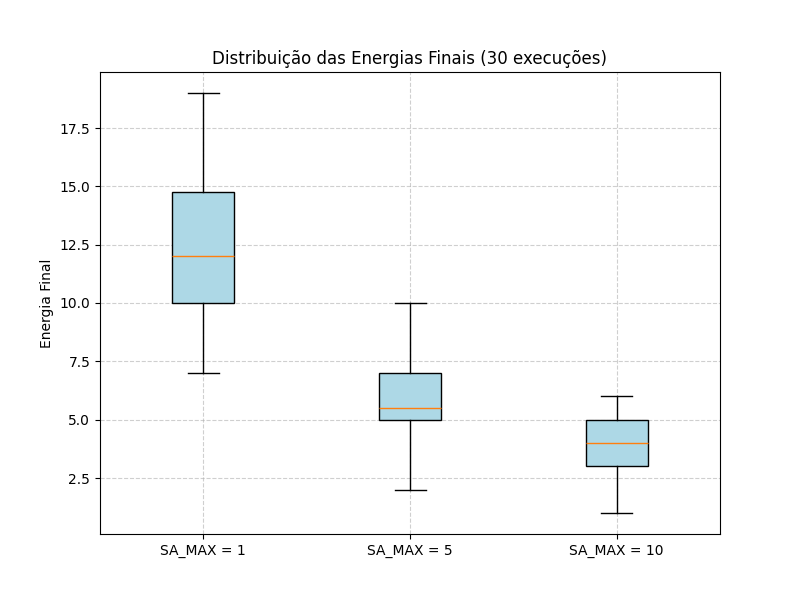
\includegraphics[width=.9\textwidth]{../../boxplot_100.png}
  \caption{Boxplots para 100 entradas}
  \label{fig:metodologia}
   \end{figure}

\begin{figure}[H]
  \centering
  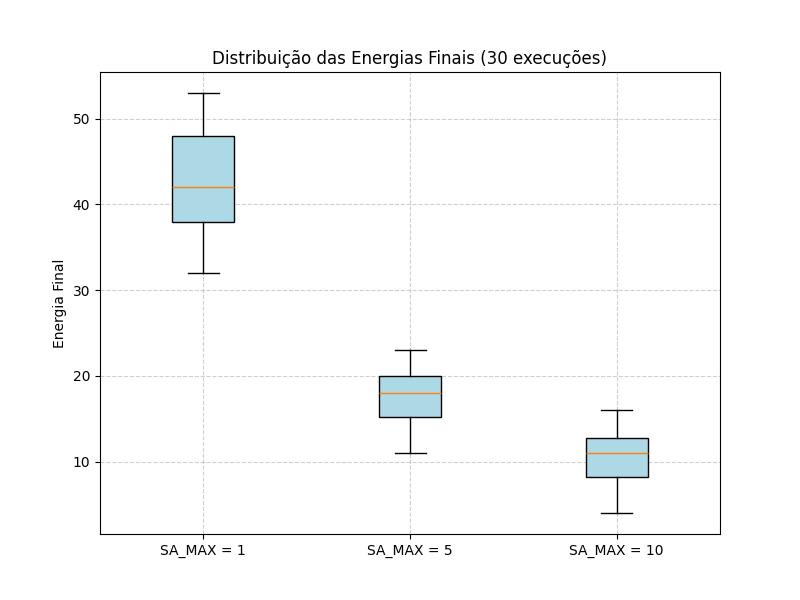
\includegraphics[width=.9\textwidth]{../../boxplot_250.png}
  \caption{Boxplots para 250 entradas}
  \label{fig:metodologia}
  \end{figure}

Dessa maneira, é possível obter uma visão aprofundada da execução do algoritmo, discutida na seção a seguir.

\section{Análise dos resultados obtidos.}
\label{sec:analise_dos_resultados_obtidos}

% Considerações sobre os resultados obtidos e análises críticas sobre os mesmos.
Factualmente, torna-se óbvia a observação de que entradas menores produzem resultados limitados, assemelhando-se mais a buscas aleatórias --- principalmente com SA\_MAX em 10 --- enquanto entradas maiores produzem resultados mais satisfatórios, com uma convergência mais acentuada.

Por outro lado, a convergência para 100 entradas, com SA\_MAX, traz resultados mais satisfatórios, com uma média de 3.93 e desvio padrão de 1.48, enquanto para 250 entradas a média é de 9.93 e desvio padrão de 2.48, como relatado na Tabela \ref{tab:resultados}.
%
Além disso, pode-se observar com os boxplots que, com o aumento do número de entradas, os resultados tornam-se mais homogêneos, relatável pelo desvio padrão, que diminui conforme o número de entradas aumenta.
Em suma, os resultados obtidos demonstram que o algoritmo de \textbf{Simulated Annealing} é capaz de resolver o problema SAT-3, com uma convergência satisfatória e resultados consistentes, principalmente para grandes entradas, tornando possível quantizar a eficiência do teorema de Gibbs, proposto em 1953.

A partir disso, surgem diversas ideias sobre o trabalho desenvolvido e direcionamentos futuros, abordados na seção a seguir.

\section{Conclusões e Trabalhos Futuros}
\label{sec:conclusoes_e_trabalhos_futuros}


Considerações sobre o trabalho desenvolvidos e identificação de direcionamentos futuros na
pesquisa.



\bibliographystyle{sbc}
\bibliography{sbc-template}

\end{document}
